% !TEX root = arbeit.tex
\section{Instrument}\label{sec:setup}
	% Pics with the lab power supply
	% \\titania.unibe.ch\UserHomes\foehn\My Documents\PhD\Fotos\[2021.02.04]FS_Sensor&Cube_in_Strofio
	\begin{figure}[h] % Prototype
		\centering
		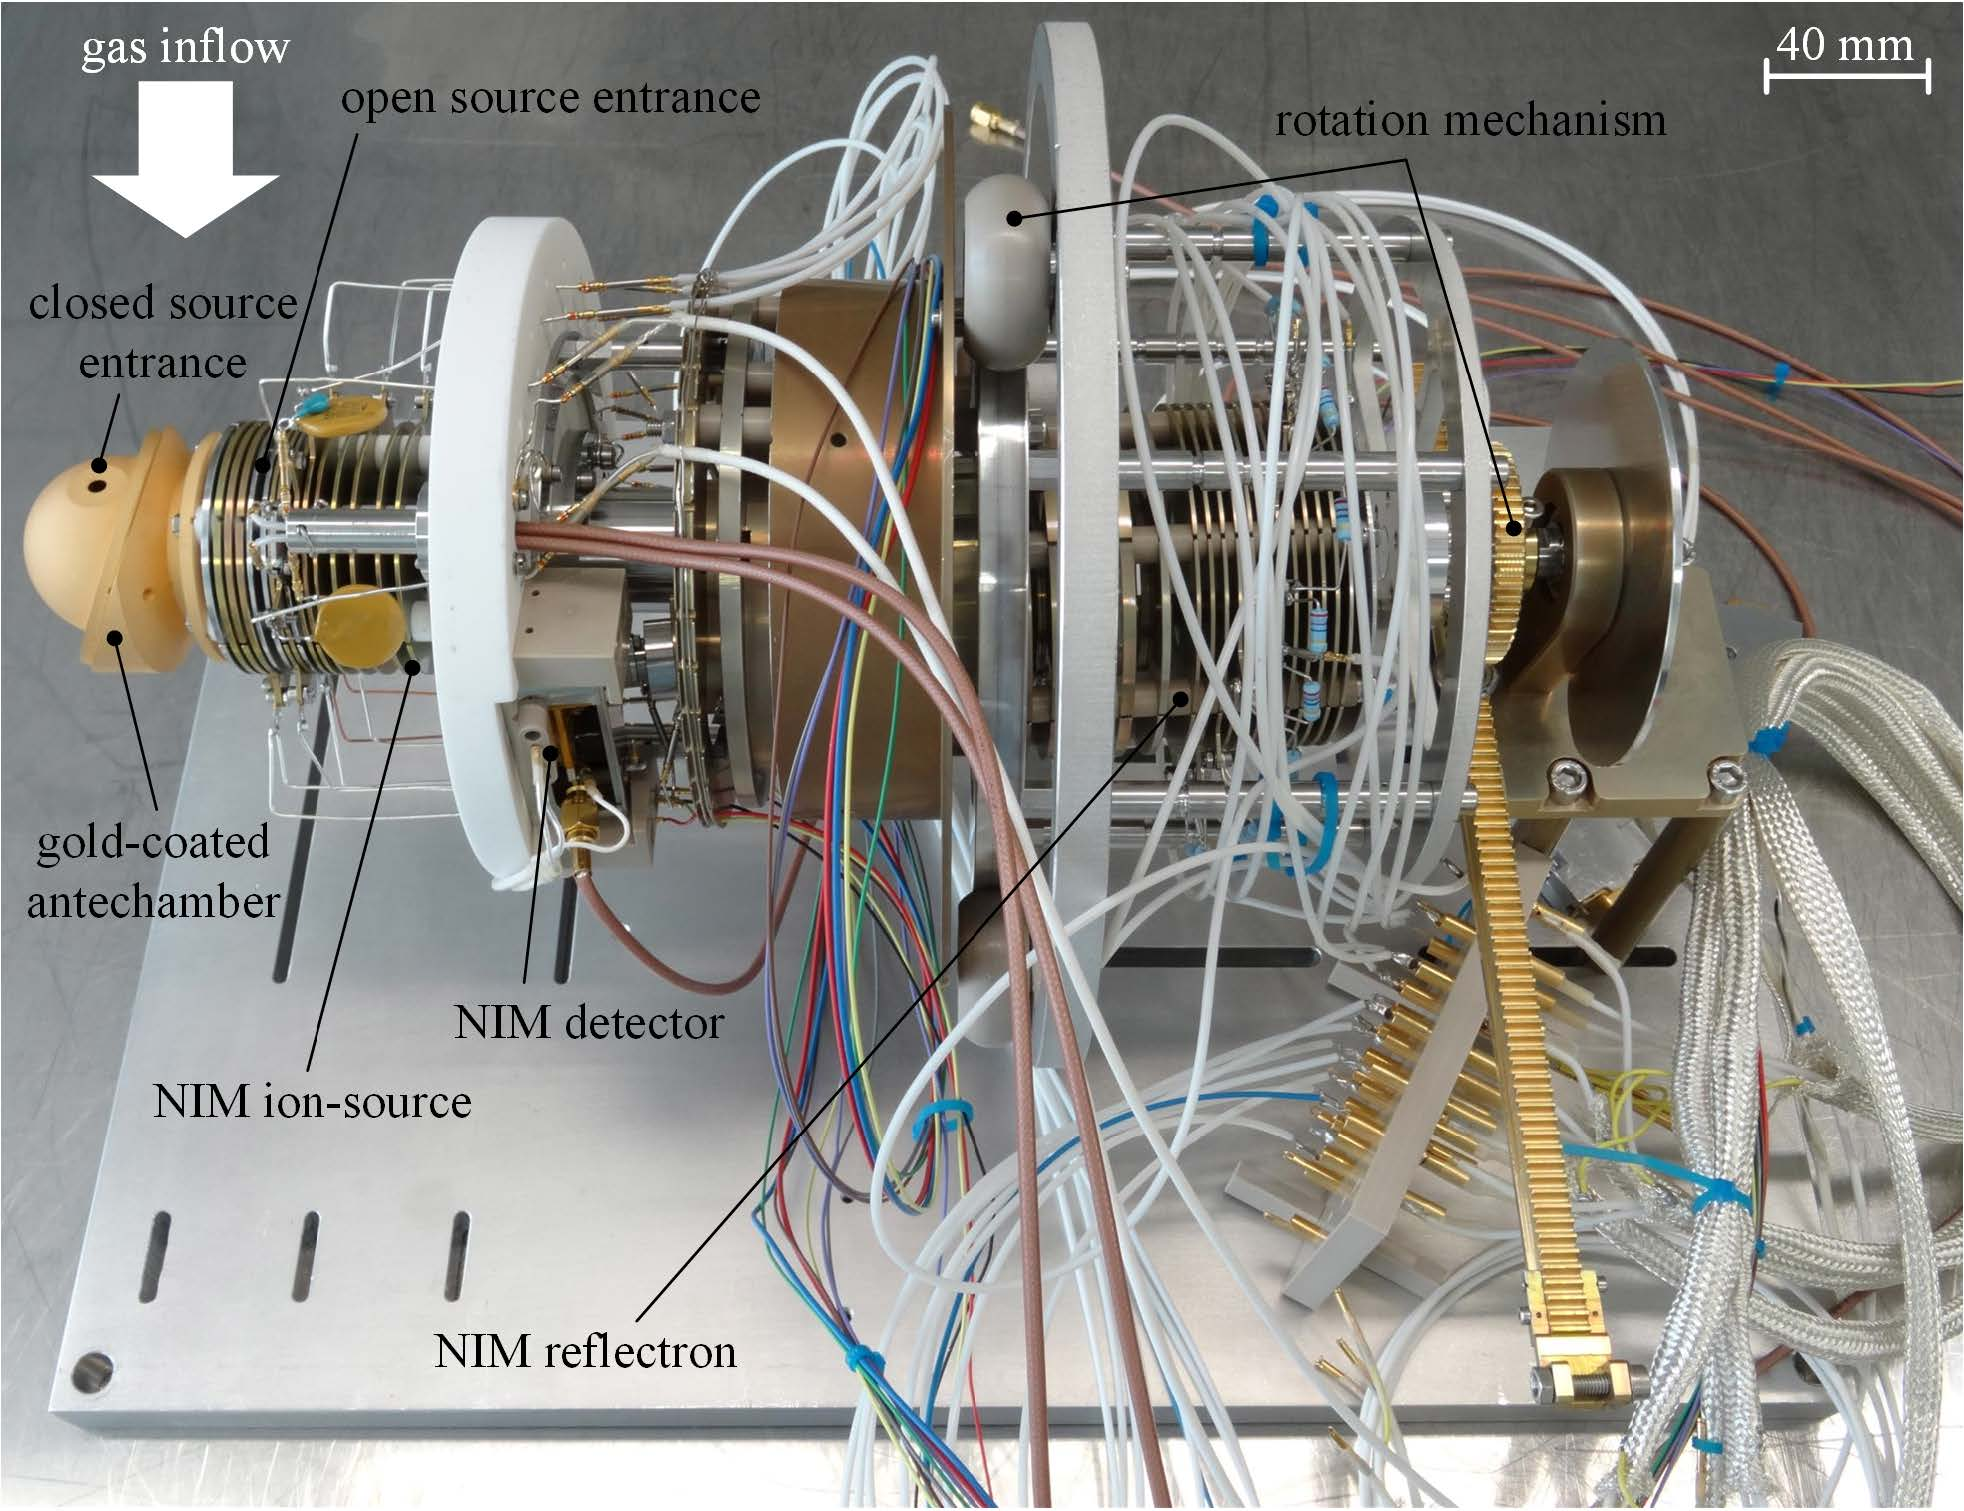
\includegraphics[width=\textwidth]{Setup/Prototype_totPic.jpg}
		\caption{The NIM Prototype \cite{Diss_Meyer}.}
		\label{fig:SetupProto}
	\end{figure}
	\begin{figure}[h] % PFM Sensor
		\begin{subfigure}{0.5\textwidth}
			\centering
			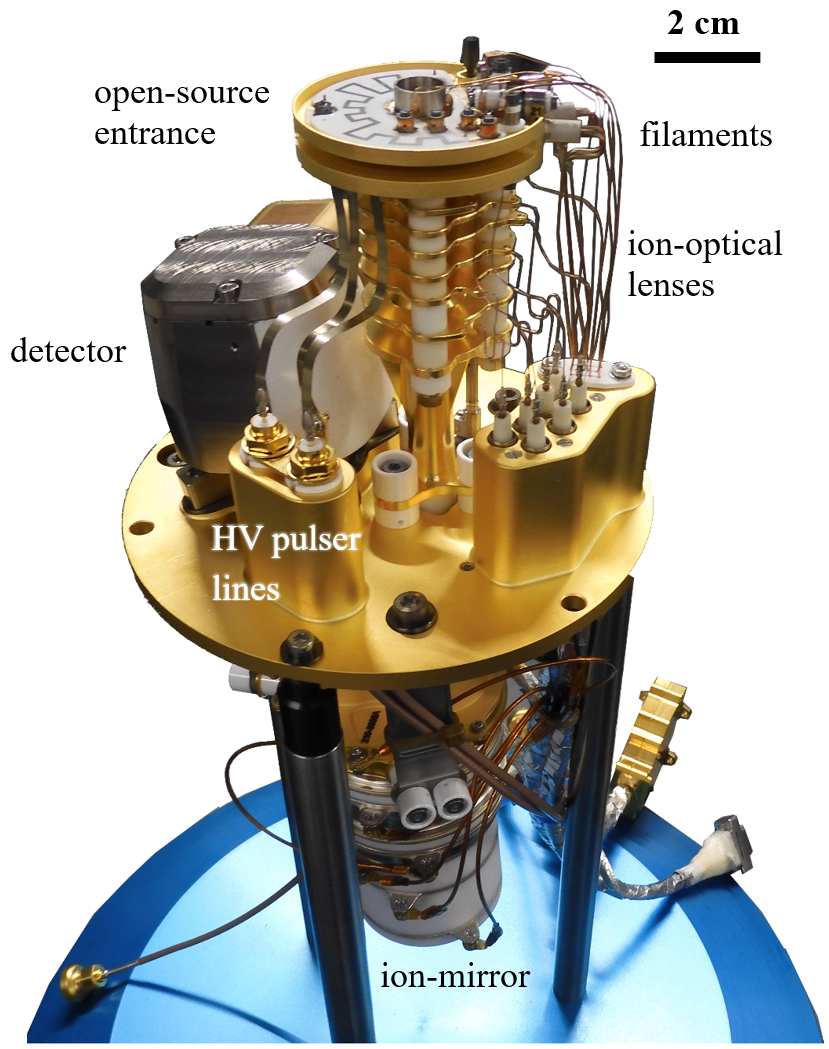
\includegraphics[width =.9\textwidth]{Setup/PFM_Sensor.png}
		\end{subfigure}
		\begin{subfigure}{0.5\textwidth}
			\centering
			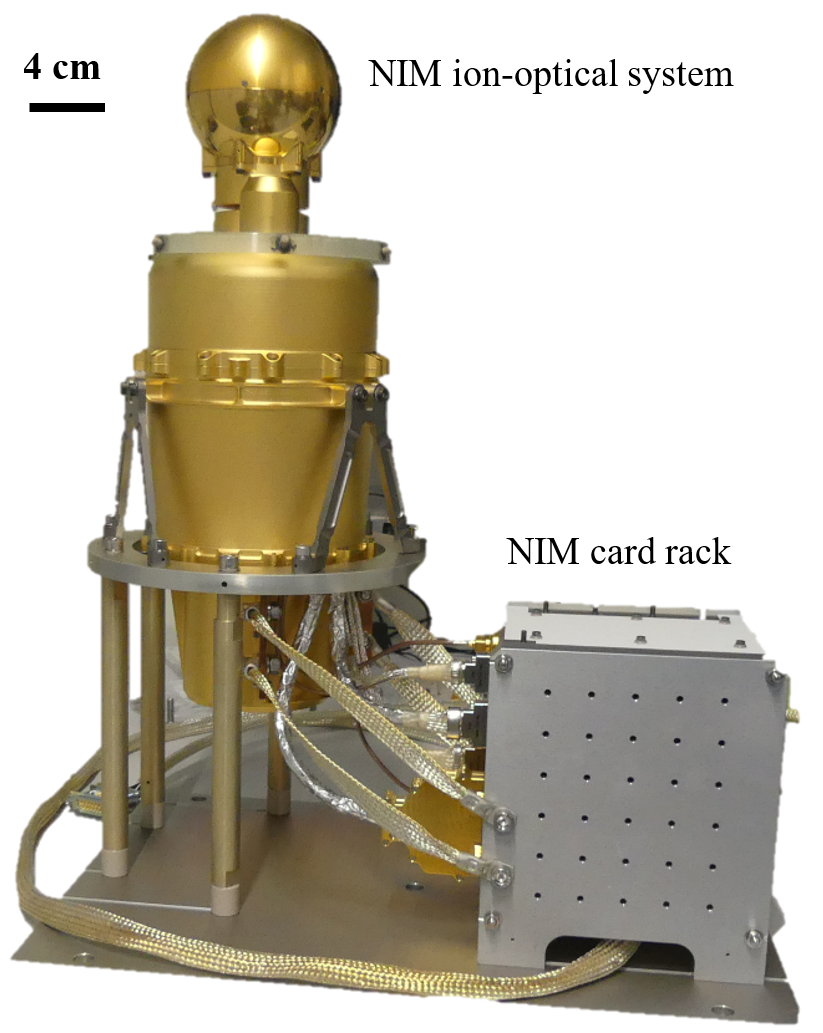
\includegraphics[width = \textwidth]{Setup/PFM_with_FlightEl.png}
		\end{subfigure}
		\caption{Left: NIM PFM ion-optical system without the antechamber and the housing. Right: The complete NIM PFM ion-optical system with electronic box (card rack) attached \cite{Foehn2021}.}
		\label{fig:SetupPFM}
	\end{figure}
	\begin{figure}[h!] % Antechamber
		\begin{subfigure}{0.5\textwidth}
			\centering
			\includegraphics[width = .9\textwidth]{Experiments/ProtoAnte.png}
		\end{subfigure}
		\begin{subfigure}{0.5\textwidth}
			\centering
			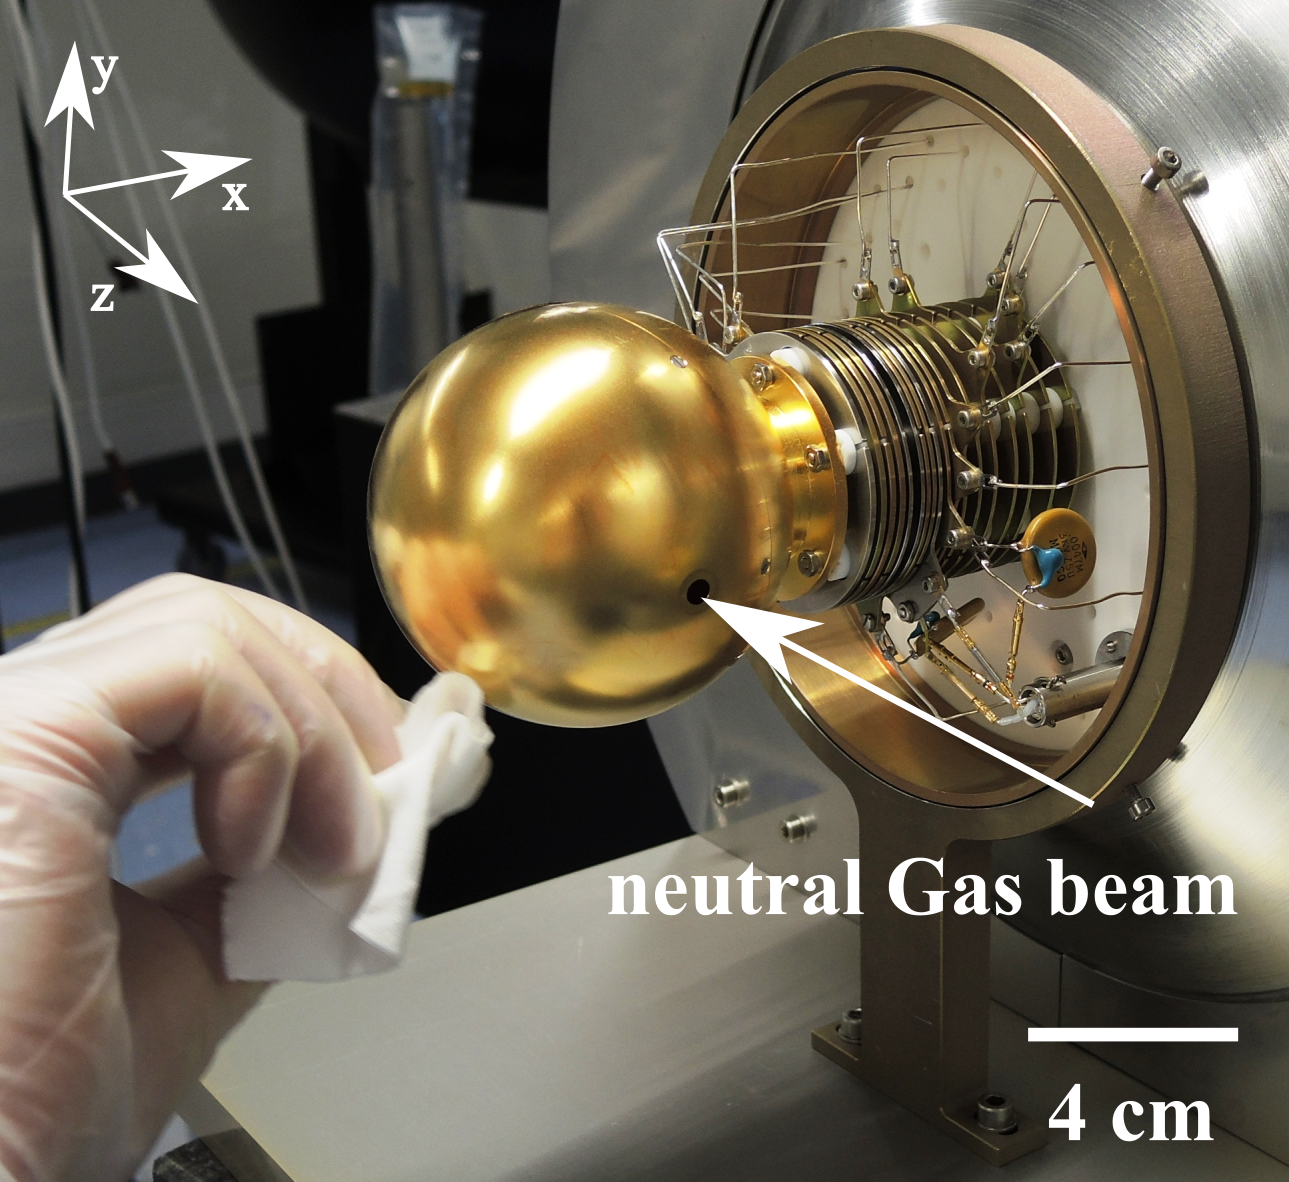
\includegraphics[width = 0.8\textwidth]{Experiments/FlightAnte.png}
		\end{subfigure}
		\caption{Left: Prototype antechamber \cite{Diss_Meyer}. Right: Flight-like antechamber. Both installed on the NIM prototype ion-optical system.}
		\label{fig:SetupAntecham}
	\end{figure}
	\begin{figure}[h] % IS Proto
		\centering
		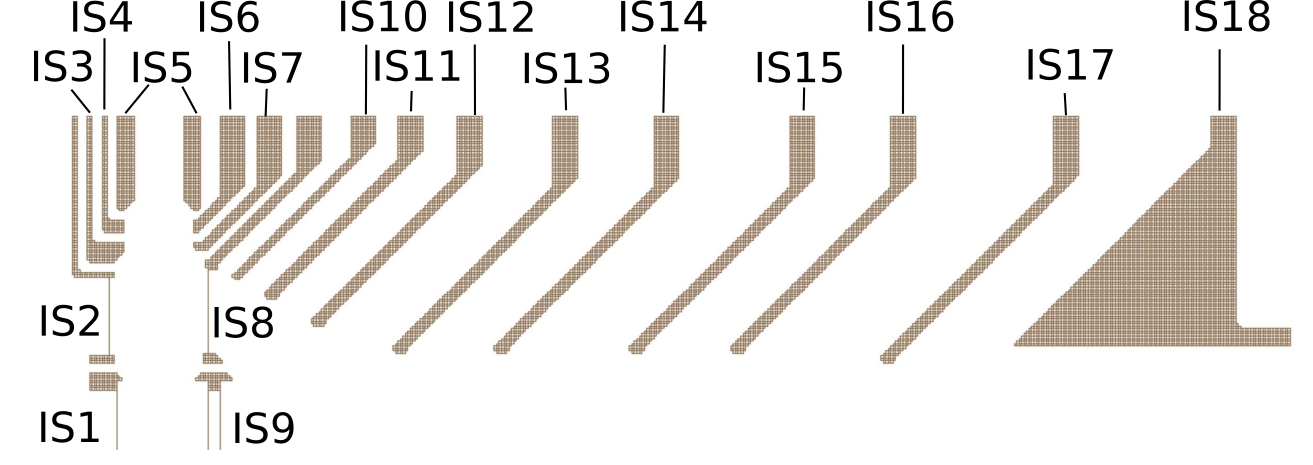
\includegraphics[width= 0.75\textwidth]{Setup/Proto_IS_sim.png}
		\caption{SIMION Model of the Ion-Source of the NIM Prototype \cite{Diss_Meyer}.}
		\label{fig:SetupProtoISSim}
	\end{figure}
	\begin{figure}[h] % IS PFM
		\centering
		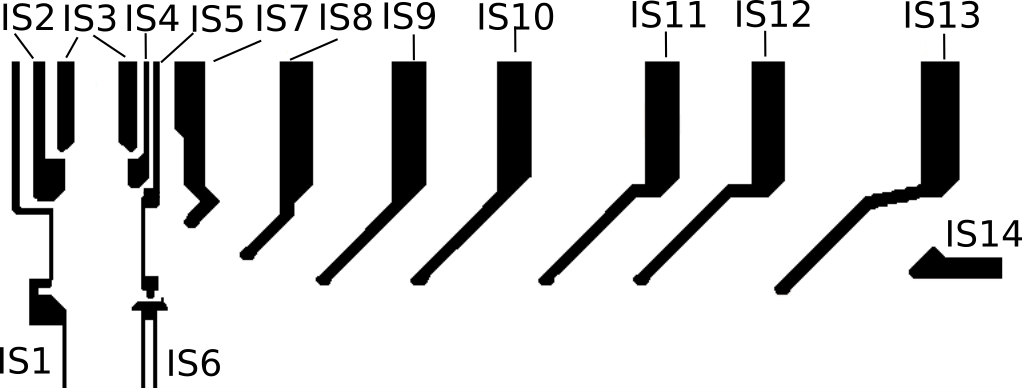
\includegraphics[width=0.7\textwidth]{Setup/ISFlight_bearb.png}
		\caption{SIMION Model of the Ion-Source of the NIM ProtoFlight Model.}
		\label{fig:SetupPFMISSim}
	\end{figure}
	\begin{figure}[h!] % Filament blocs
		\begin{subfigure}{0.5\textwidth}
			\centering
			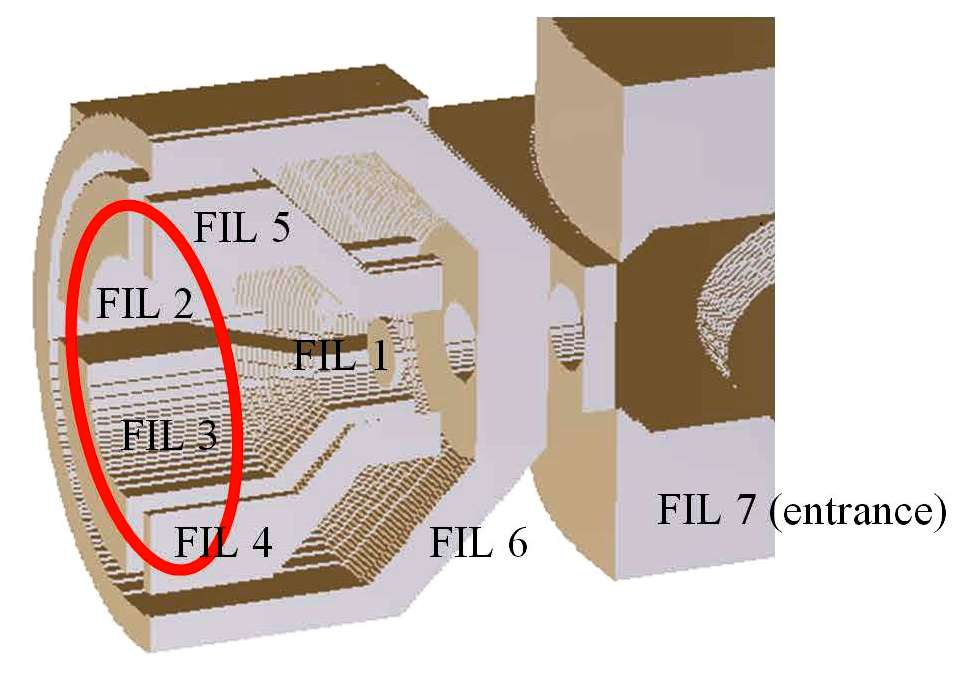
\includegraphics[width =0.85\textwidth]{Setup/Proto_FilEl_sim.jpg}
		\end{subfigure}
		\begin{subfigure}{0.5\textwidth}
			\centering
			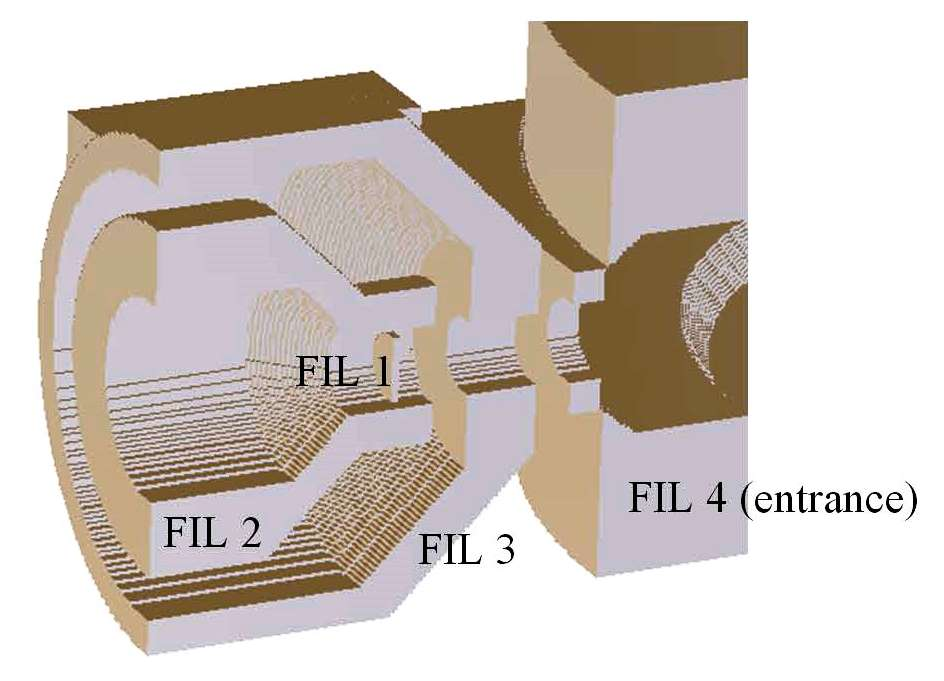
\includegraphics[width = 0.85\textwidth]{Setup/PFM_FilEl_sim.jpg}
		\end{subfigure}
		\caption{Left: Prototype filament housing \cite{Diss_Meyer}. Right: PFM filament housing \cite{Diss_Meyer}.}
		\label{fig:SetupFilElSim}
	\end{figure}
	
	This chapter compares the NIM prototype (Fig.~\ref{fig:SetupProto}) with the NIM ProtoFlight Model (PFM) (Fig.~\ref{fig:SetupPFM}) from the mechanical point of view. The NIM prototype was developed in the thesis of Stefan Meyer \cite{Diss_Meyer}, and is a complete ion-optical realisation of the system. However, the mechanical design is just for laboratory use, and is not suitable for flight.\\
	The NIM PFM instrument is the flight realisation of this ion-optical system, with some simplifications and optimisations. In Fig.~\ref{fig:SetupPFM}, left panel, the ion-optical system of the PFM is shown, and in the right panel the entire NIM PFM is shown, with the ion-optical system inside the housing and the operating electronics in their separate radiation shielded box. Comparing Fig.~\ref{fig:SetupProto} and Fig.~\ref{fig:SetupPFM} shows the key differences between the two models. Special focus lay hereby on the design of the detector because there were made some major design improvements.\\
	Fig.~\ref{fig:SetupAntecham}~left shows the prototype antechamber and right the PFM antechamber. To improve the performance of the antechamber, the flight antechamber was made twice as big as the old one of the prototype. In addition, it has two entrance holes at $\pm$30° relative to the x-axis of the instrument to be able to measure gas coming from both directions of the instrument (see Chap~\ref{subsubsec:Calfly}). Since the flight version has two entrance holes and the interface to the ion-source contains a shutter, a larger surface area of the antechamber was needed to compensate for the openings. % (A\textsubscript{surface} > 100$\sum$A\textsubscript{holes}).
	The main inflow direction of the neutral particle beam generated by the CASYMIR test facility is 90° \cite{CASYMIR_Graf2004}. Therefore, a second flight-like test antechamber was made which has the second entrance hole at position 90° to be able to test the flight antechamber.\\
	The antechambers consists of two parts which are hold together with screws. Tests of the prototype antechamber revealed that two of the mounting screws generate signal artefacts \cite{Meyer_2017_ante}. Therefore, the outer surface of the antechamber was redesigned (see also Chap.~\ref{subsec:ExpAnteCham}).\\
	Fig.~\ref{fig:SetupProtoISSim} shows the SIMION model of the Prototype ion-source, Fig.~\ref{fig:SetupPFMISSim} shows the ion-source of the PFM and Fig.~\ref{fig:SetupFilElSim} shows the filament housing of the Prototype (left) and of the PFM (right). The PFM ion-source has seven electrodes less then the prototype to simplify the source and the flight electronics, in particular to reduce the number of high voltages needed. Several low-voltage electrodes were taken together such as IS~1 and IS~2, IS~3 and IS~4 and IS~6 and IS~7. IS~10 was removed and IS~11 was shifted towards the ionisation region.\\
	In the filament housing the electron repelling electrodes Fil~2~--~Fil~5, which served to stear the electron beam through the ionisation region, were taken together to one single electrode Fil~2. The electron repelling electrode in the prototype was split into four parts to compensate with the electric fields for a bad alignment of the filament. For the PFM, the mounting of the filament holder was improved and therefore these four electrodes could be taken together to one single electrode.\\
	\begin{figure}[h!] % ion mirror
		\centering
		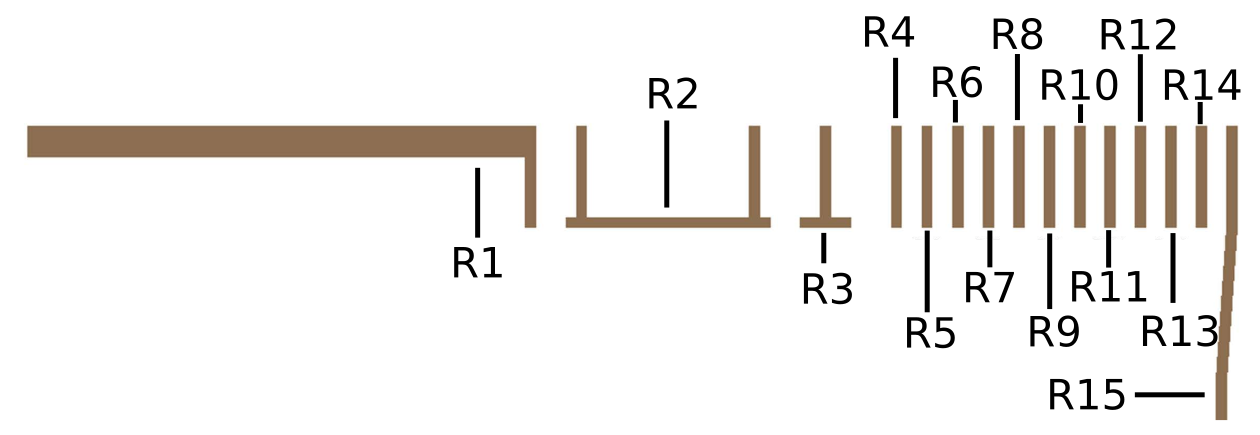
\includegraphics[width=0.9\textwidth]{Setup/Prototype_Reflectron_sim.png}
		\caption{SIMION Model of the ion-mirror of the NIM Prototype \cite{Diss_Meyer}.}
		\label{fig:SetupProtoReflSim}
	\end{figure}
	Fig.~\ref{fig:SetupProtoReflSim} shows a schematics of the ion-mirror. The prototype ion-mirror consists of 14 ring-electrodes (R~2~--~R~15) to establish a potential gradient. Electrode R~1 is the drift tube. R~2 is the ion-mirror lens electrode, R~3 is on drift potential. The set R~1-R~2-R~3 establishes a thick lens (similar to geometric optics). Electrodes R~4~--R~25 establish the actual ion-mirror. Between the electrodes R~4~--~R~15 are resistors to connect the electrodes with each other to generate a linear voltage gradient when a voltage is applied at electrodes R~4 and R~15. In addition, a voltage can be applied on electrode R~8 allowing additional focusing of the ions within ion-mirror. The flight version of the ion-mirror consists of a ceramic tube with two resistance spirals on its inner walls replacing electrodes R~5~--~R~7 and R~9~--~R~14 respectively. From the electrical and ion-optical point of view, the two ion-mirrors behave the same.\\
	% Detector Figs.	
	\begin{figure}[h!] % Photograph of the Prototype an Flight detector.
		\begin{subfigure}{0.5\textwidth}
			\centering
			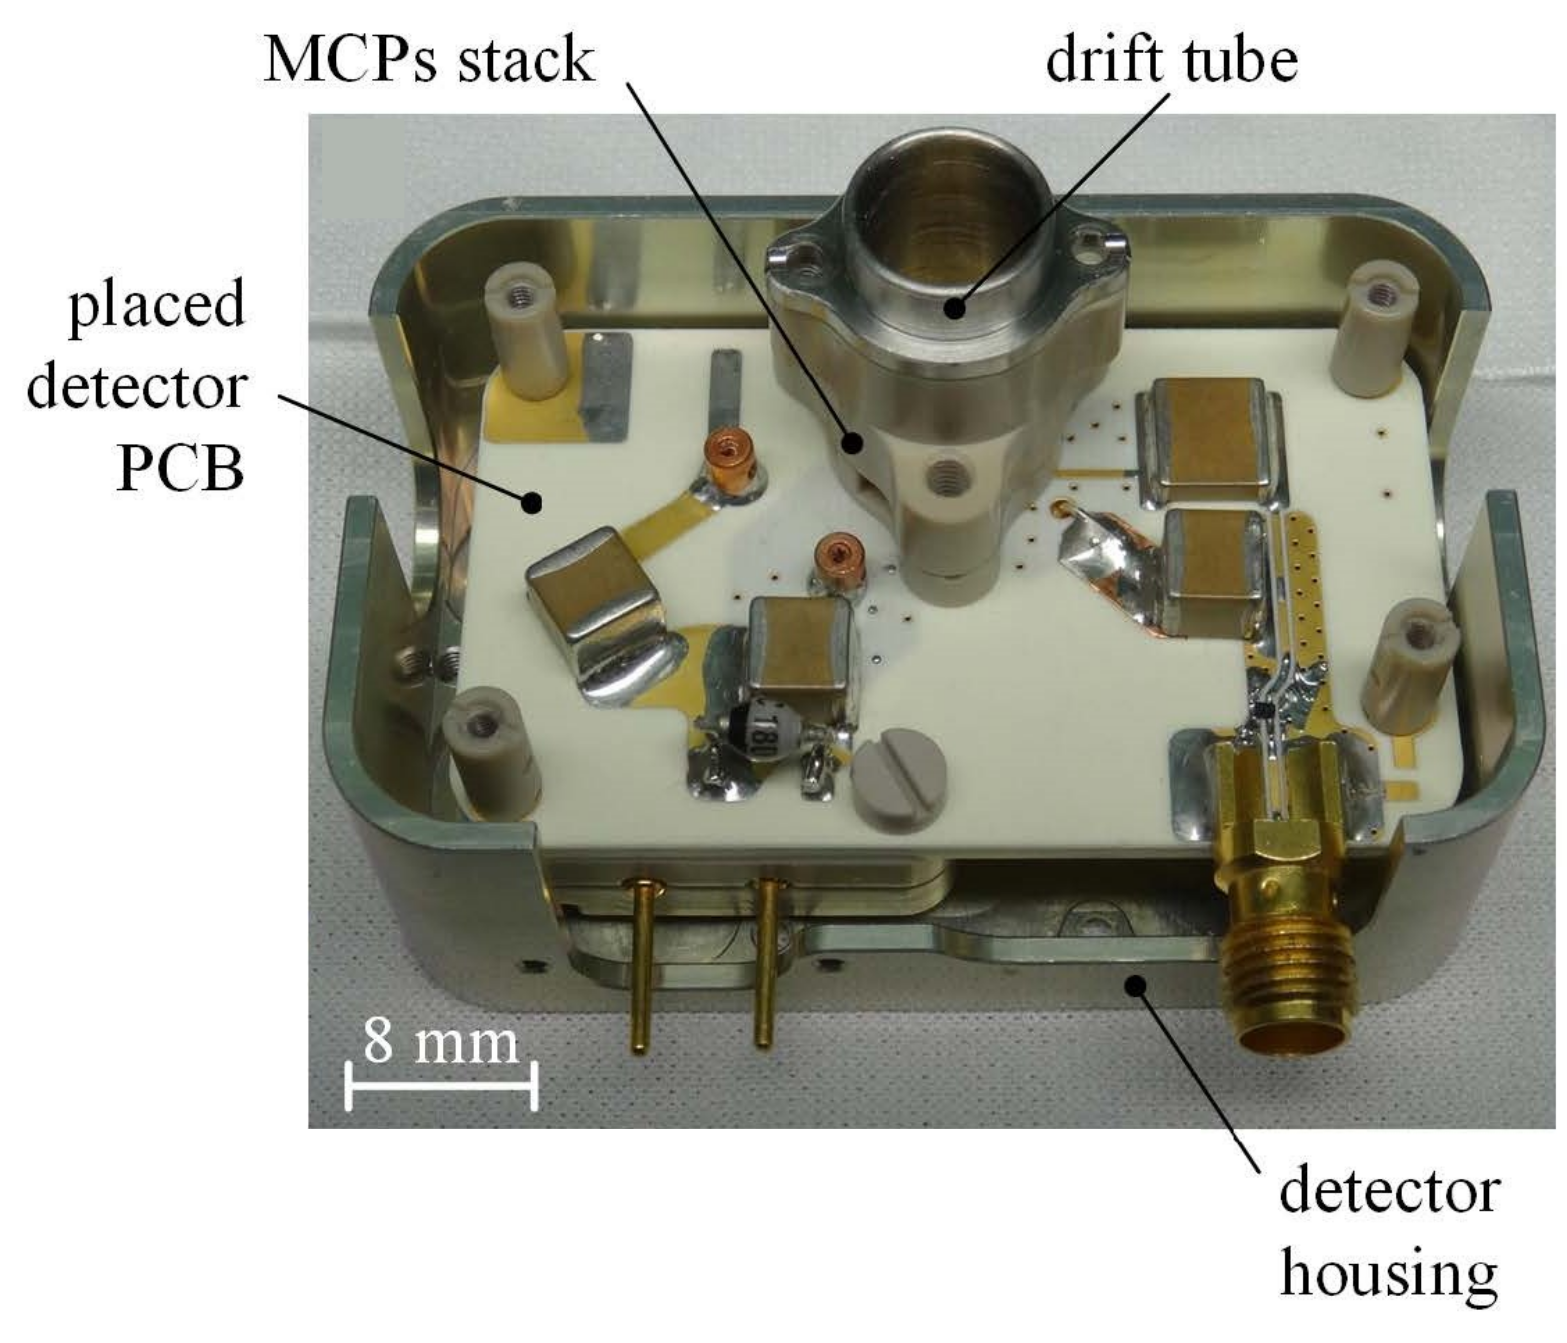
\includegraphics[width=\textwidth]{Setup/Prototype_Detector.png}
		\end{subfigure}
		\begin{subfigure}{0.5\textwidth}
			\centering
			\includegraphics[width=.9\textwidth]{Setup/Flight_Detector.png}
		\end{subfigure}
		\caption{Left: NIM Prototype detector \cite{Diss_Meyer}. Right: NIM Flight detector without its radiation shield.}
		\label{fig:DetPhotos}
	\end{figure}
	\begin{figure}[h!]
		\centering
		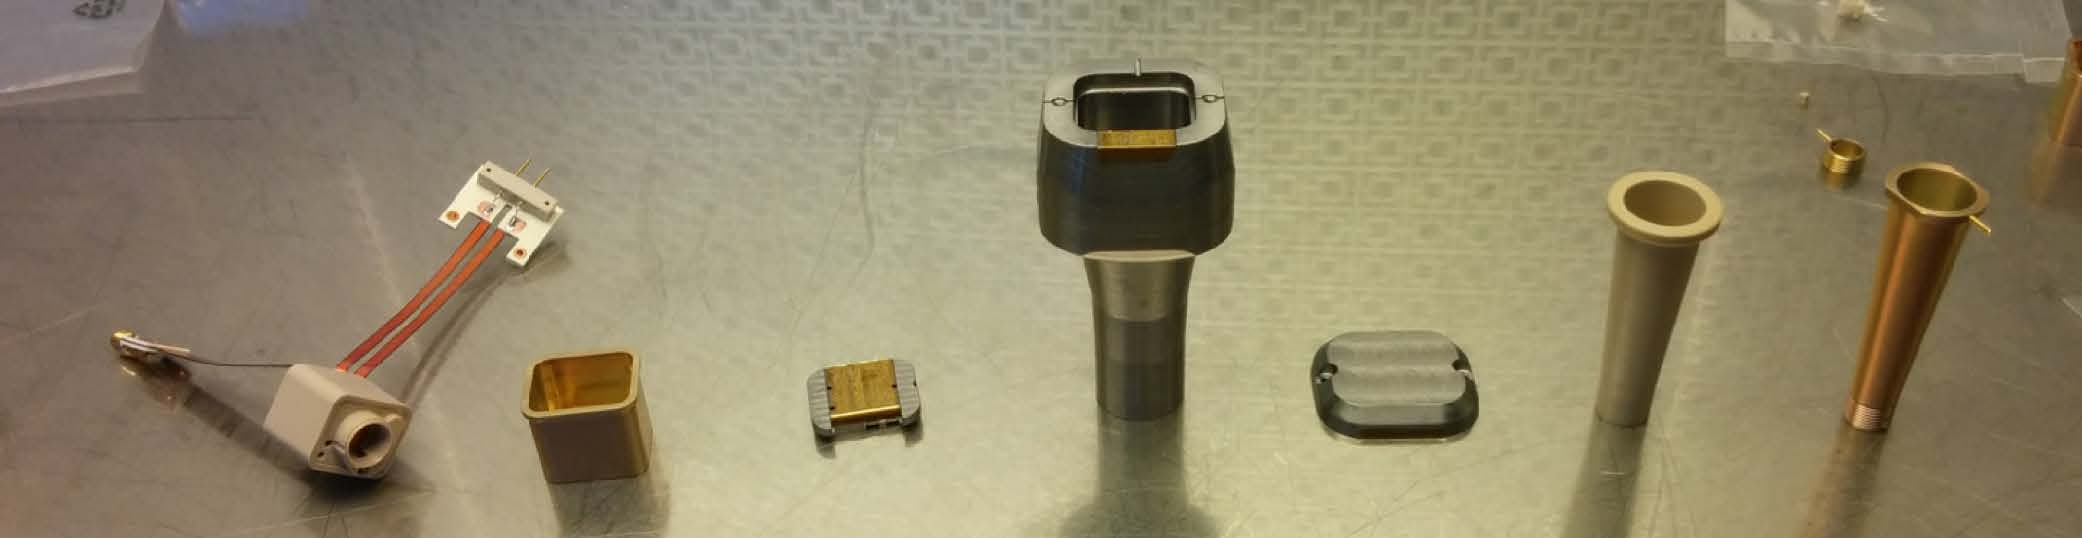
\includegraphics[width=\textwidth]{Setup/PFM_Det_Shield.jpg}
		\caption{Components of the NIM flight detector. From left to right: Detector folded in PEEK housing, Al cover, Ta shielding, PEEK drift tube to electrically isolate the Al drift tube from the shielding \cite{Lasi_2017_Detector}.}
		\label{fig:DetShield}
	\end{figure}
	\begin{figure}[h] % Schematics of the 2 detector designs.
		\centering
		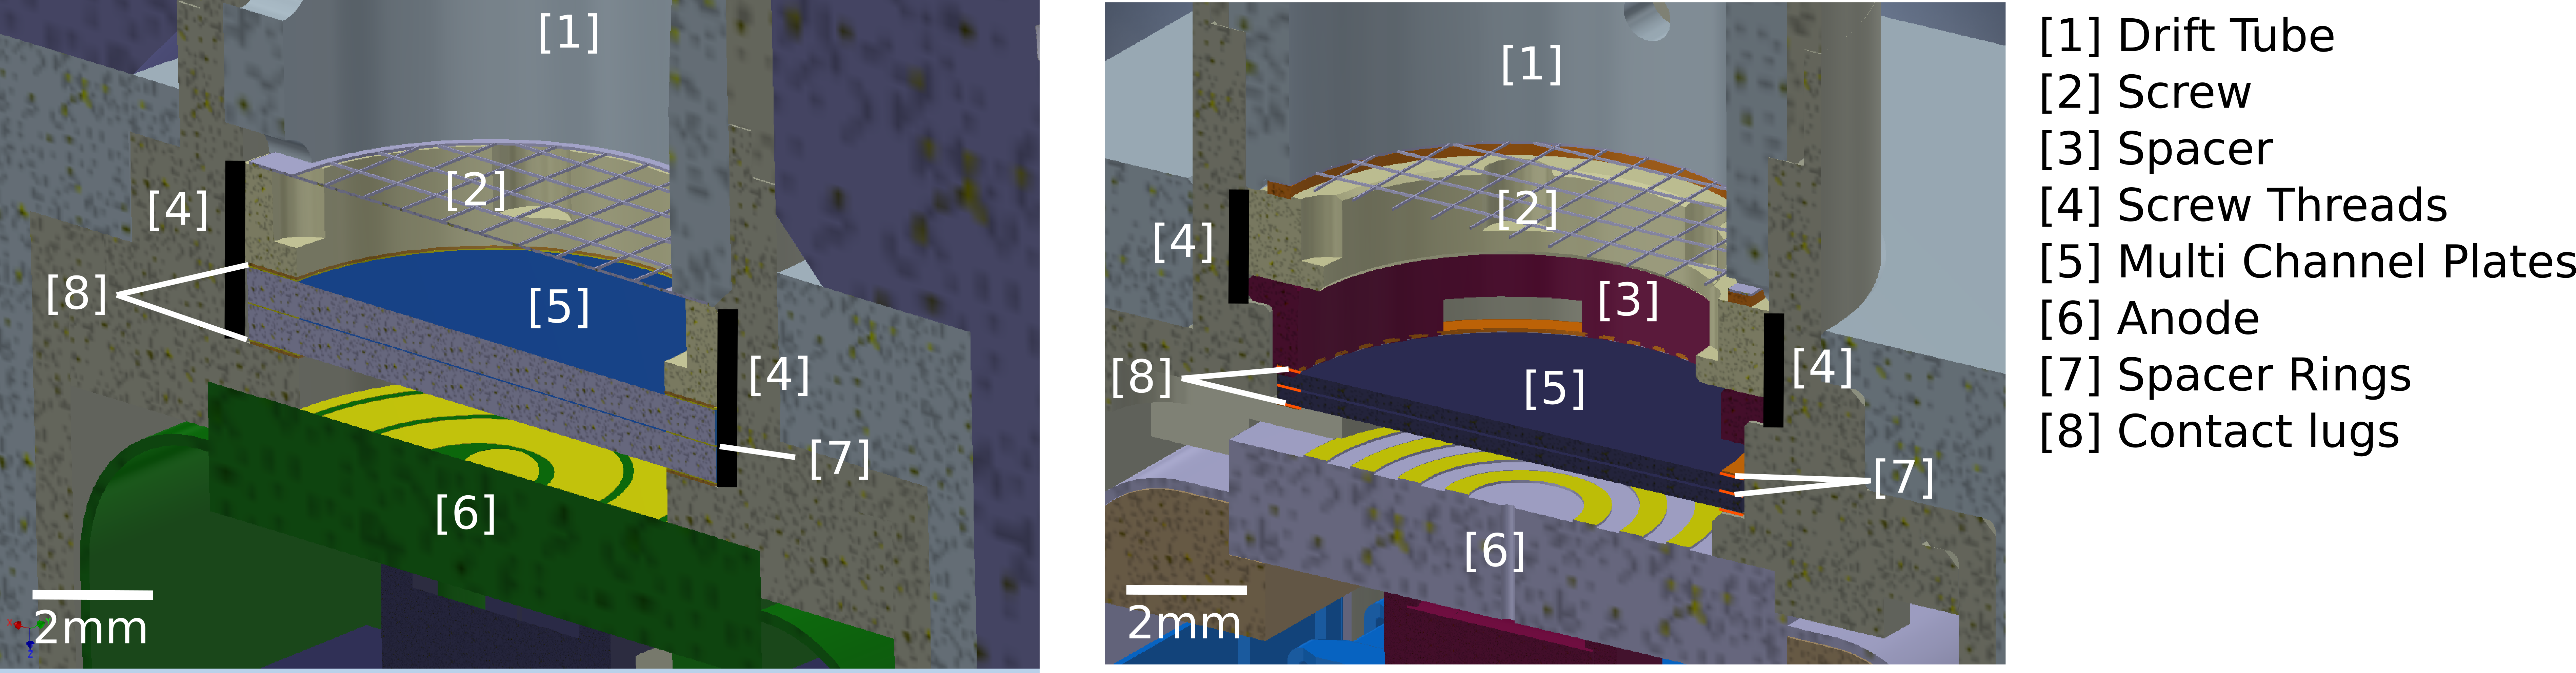
\includegraphics[width= \textwidth]{Setup/PFMDetectors.png}
		\caption{Schematics of the PFM detector housings. Left: preliminary design. Right: final flight design.}
		\label{fig:FlightDetSchemata}
	\end{figure}
	\begin{figure}[h] % Circuit diagram
		\centering
		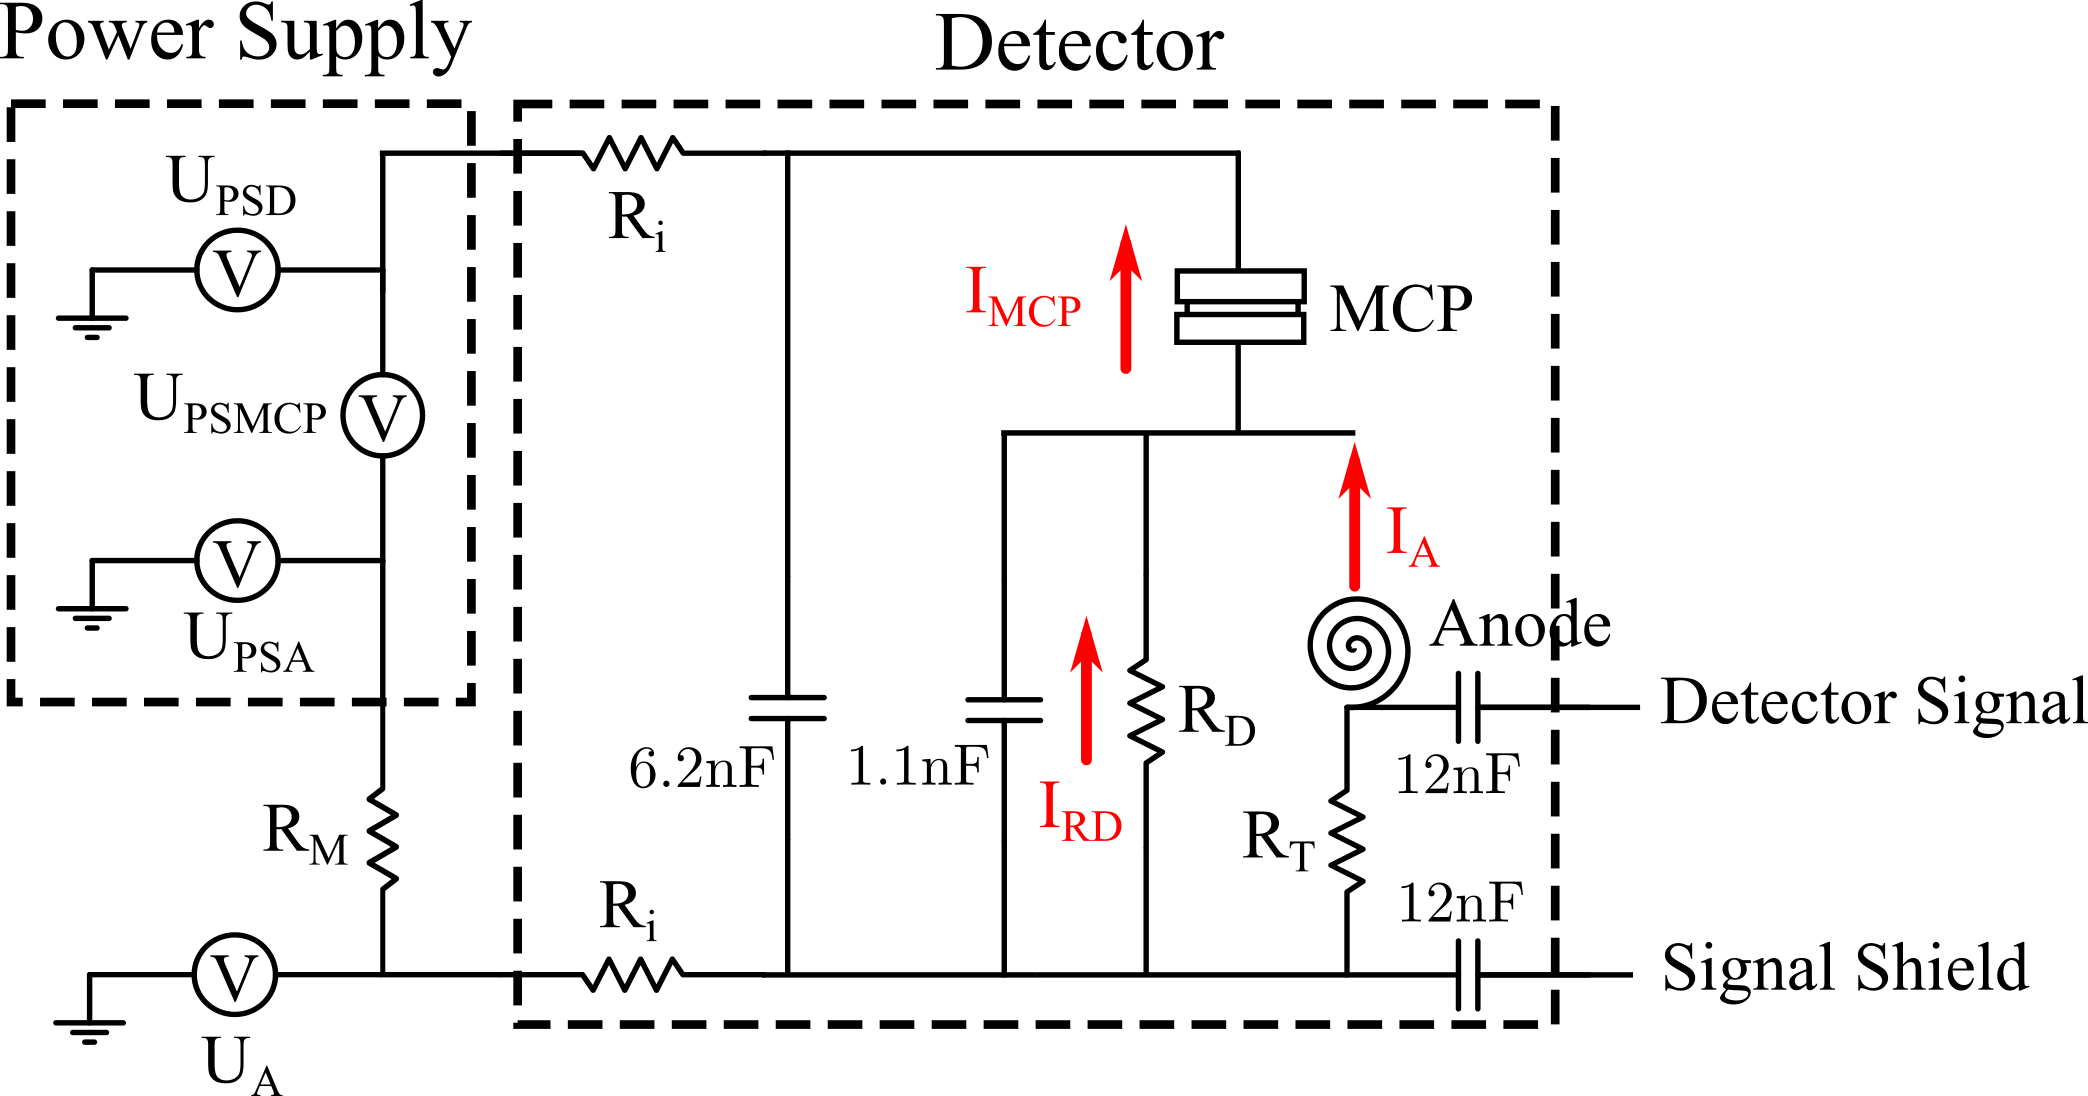
\includegraphics[width = \textwidth]{Bilder/Detector_elec_schema.png}
		\caption{Electrical schematics of the NIM flight detector with laboratory electronics attached.}
		\label{fig:FlighElecSchema}
	\end{figure}
	% free play = technisch Spiel. Put it in during proofreading.
	The NIM Prototype detector has a rigid Printed Circuit Board (PCB) on which the electrical components and the drift tube adapter with the MCP stack are mounted (Fig.~\ref{fig:DetPhotos}~left panel and Fig.~\ref{fig:DetShield}). Due to Jupiter's strong radiation field, the detector has to be shielded to reduce the noise level induced by the strong radiation and to increase the detector's lifetime. To minimise the required shielding mass, the flight detector has to be very compact. This was achieved by using a flex PCB to fold the detector into a PEEK housing (Fig.~\ref{fig:DetPhotos}, right panel).\\ Fig.~\ref{fig:FlightDetSchemata}, left panel shows the mechanical design of a preliminary design of the PEEK housing containing the MCPs. The MCPs lay on a ledge 1~mm above the anode. A Zener diode generates a voltage between the MCP backside and the anode to accelerate the electrons from the MCP backside towards the anode (see electrical scheme Fig.~\ref{fig:FlighElecSchema}). There are two contact lugs on top and at the bottom of the MCP stack to apply a voltage over the MCPs. The MCPs are fixed with a PEEK screw within the housing. In the old design, the screw threads were milled down to the ledge. When the MCPs were mounted, they often canted in the threads. In addition, it was not possible to determine, how much the screw had to be tightened. When the screw was tighten too much, the MCPs broke as they consist of lead glass and are therefore very fragile. When the screw was too loose, the two contact lugs had no reliable electrical contact to the MCPs. When applying a high voltage over the whole MCP stack, the gaps between the contact lugs and the MCPs act as an additional resistors over which the voltage builds up resulting in a discharge between the electrodes and the MCPs. The discharge can propagate through the whole MCP stack and damages the readout electronics. As a consequence, the screw thread was milled less far and an additional mechanical stop was made to tighten the screw only down to that stop (Fig.~\ref{fig:FlightDetSchemata}, right panel). This prevented the MCPs from canting in the screw thread thus it was not milled down to the bottom of the lower ledge and with the mechanical stop, the screw could not be tightened too much to break the MCPs. In addition, a PEEK spacer was added between the screw and the MCPs to push down the MCPs uniformly. Due to the mechanical tolerances in the manufacturing process of the different parts of the housing, metallic spacer rings are added between the PEEK spacer and the contact lug of the top MCP to close the resulting gap. The number of added rings varies between each detector because the gap resulting from the varying mechanical tolerances is different for each manufactured housing. With this design, the electrical contact between the MCPs and the contact lugs could be improved but from the electrical point of view its still not a reliable electrical contact.\\
	To make the system more robust against discharges the Zener diode was exchanged through a resistor ($R_D$ in Fig.~\ref{fig:FlighElecSchema}). The flight electronics sets the voltage $U_{stack}$ between the top MCP and the anode. The MCPs and the Zener diode act as voltage dividers, which are connected in series. Therefore, the potential drop over the MCPs depends on the potential drop over the Zener diode. The voltage drop over the Zener diode is 180~V independent of $U_{stack}$. Therefore, the voltage over the MCPs $U_{MCP}$ is 180~V lower than $U_{stack}$. When having a resistor $R_D$ instead of a Zener diode, the voltage over the MCPs cannot be calculated by just having $U_{stack}$ because the resistance of the MCPs $R_{MCP}$ depends on the voltage $U_{MCP}$ applied over them. The resistance also changes with time due to ageing because the conductive material inside the MCP channels degrades over time. Therefore, the current $I_{MCP}$ flowing through the system has to be known to be able to calculate $U_{MCP}$. The NIM flight electronics is not designed to measure this current because it was designed for a detector with a Zener diode where a current measurement would be unnecessary. A calibration with the laboratory electronics was done to determine the relationship between $U_{stack}$ and $U_{MCP}$ (Chap.~\ref{chapExp:Det}).\\
	In the following section, $U_{MCP}$ is derived as a function of the different voltages known when measuring with laboratory electronics. Fig.~\ref{fig:FlighElecSchema} shows the circuit diagram of the detector when operated with laboratory electronics and Table~\ref{tab:ElecSchemaVariableList} summarizes the used variables. The current flowing through the MCPs $I_{MCP}$ is measured with the resistor $R_M$:
	\begin{equation}
		I_{MCP} = \frac{U_{RM}}{R_{M}}
	\end{equation}
	With $U_{RM}$ the voltage over the resistor $R_{M}$ which is:
	\begin{align}
		U_{RM} &= U_{PSA} - U_{A}\\
			   &= U_{PSMCP} + U_{PSD} - U_A
	\end{align}
	With $U_{PSA}$ the power supply output voltage for the anode, $U_{A}$ the voltage applied on the detector anode, $U_{PSD}$ the power supply output voltage applied at the top contact lug of the MCP stack and $U_{PSMCP}$ the voltage difference between the two power supply outputs. $U_{PSMCP}$ is:
	\begin{equation}
		U_{PSMCP} = U_{RM} + 2\cdot U_{Ri} + U_{RD} + U_{MCP}
		\label{eq:UpsmcpTot}
	\end{equation}
	With $U_{Ri}$ the voltage over the input resistors $R_i$, which are there to damp noise coupled into the detector circuit from the power supply:
	\begin{equation}
		U_{Ri} = I_{MCP}\cdot R_i
	\end{equation} 
	$U_{RD}$ is the voltage over the resistor $R_D$ replacing the former diode. The current $I_A$ induced when an ion generates an electron avalanche, is very low compared to the current $I_{RD}$. Therefore, $I_{MCP} = I_{RD}$ and:
	\begin{equation}
		U_{RD} = I_{MCP}\cdot R_D
	\end{equation}
	Solving Eq.~\eqref{eq:UpsmcpTot} for $U_{MCP}$ and inserting the different voltages results in:
	\begin{align}
		U_{MCP} =& U_{PSMCP} - U_{RM} - 2\cdot U_{Ri} - U_{RD}\\
				=& U_{PSMCP} - U_{PSMCP} + U_{PSD} - U_A - 2\cdot I_{MCP} R_i - I_{MCP} R_D\\
				=& (U_A - U_{PSD})\cdot\left(1 + \frac{2R_i + R_D}{R_M}\right) - U_{PSMCP}\frac{2R_i + R_D}{R_M}
	\end{align}	
	The measurements with this setup (Fig.~\ref{fig:FlighElecSchema}) of the MCP voltage and resistance are presented below, in Chap.~\ref{chapExp:Det}.
	
	\begin{table}[h]
		\begin{center}
		\begin{tabular}{|m{1.5cm}|m{5.4cm}|m{1.5cm}|m{5.4cm}|}
			\hline
			R\textsubscript{D}& Resistor replacing the former diode & U\textsubscript{A}& Voltage on the detector anode \\
			R\textsubscript{i} & Detector input resistor & U\textsubscript{MCP}& Voltage over the MCPs \\
			R\textsubscript{M}& Resistor used to determine I\textsubscript{MCP} &U\textsubscript{PSA} & Anode voltage output of power supply \\
			R\textsubscript{MCP}& MCP resistance & U\textsubscript{PSD} & Drift voltage output of power supply \\
			R\textsubscript{T} & 50~$\Omega$ termination & U\textsubscript{PSMCP} & Voltage difference  between U\textsubscript{PSA} and U\textsubscript{PSD} \\
			I\textsubscript{A} & Current induced in the MCPs when an ion hits the MCPs & U\textsubscript{RD}& Voltage over R\textsubscript{D} \\
			I\textsubscript{ion} & Ion current hitting the MCPs & U\textsubscript{Ri}& Voltage over R\textsubscript{i} \\
			I\textsubscript{MCP} & Current flowing through the MCPs &U\textsubscript{RM}& Voltage over test resistor R\textsubscript{M}\\
			I\textsubscript{RD} & Current flowing through R\textsubscript{D} &&\\
			\hline
		\end{tabular}
		\end{center}
		\caption{List of the variables used in the schematics of the flight detector Fig.~\ref{fig:FlighElecSchema} when the detector is operated with laboratory electronics.}
		\label{tab:ElecSchemaVariableList}
	\end{table}
	\begin{figure}[h!]
		\centering
		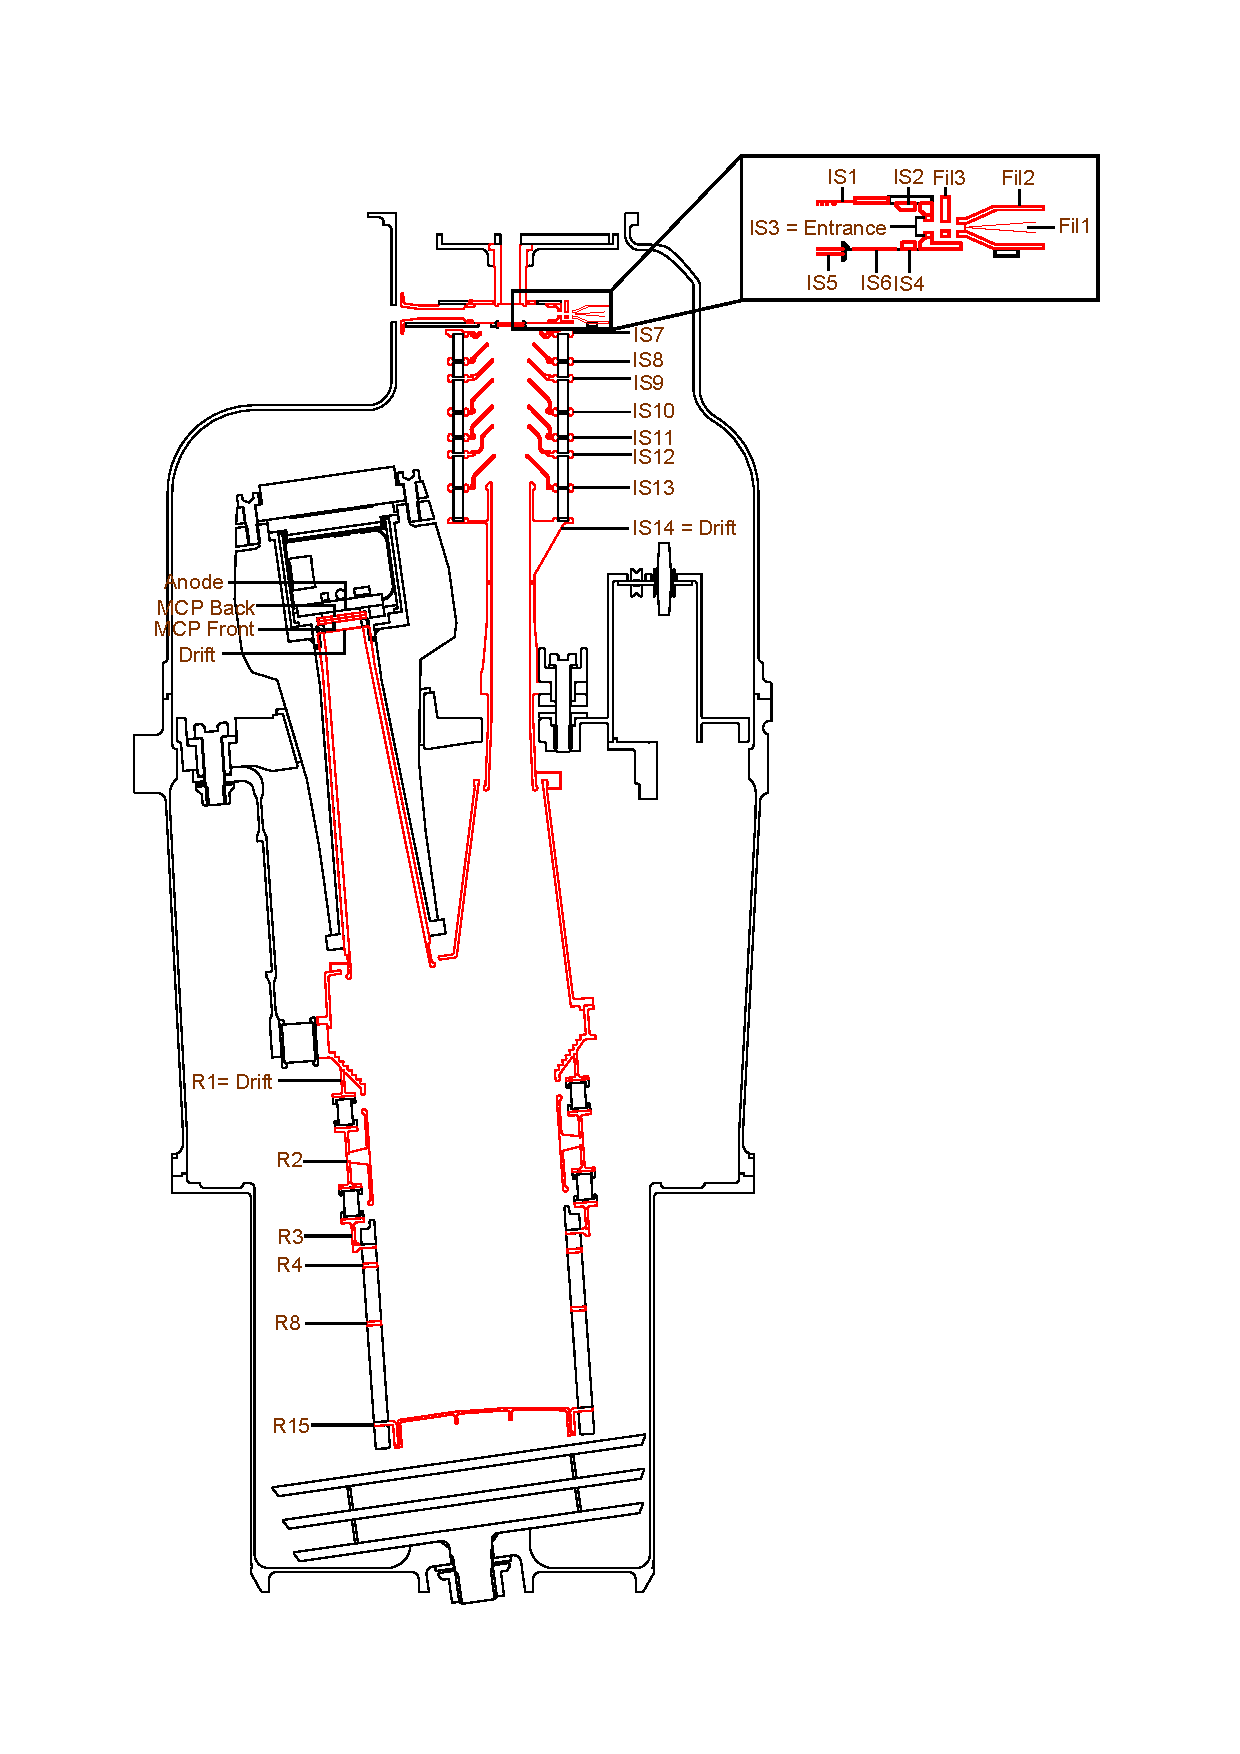
\includegraphics[width= 0.9\textwidth]{Setup/NIM_schema.pdf}
		\caption{Schematics of the NIM flight design with all electrodes of the ion-optical system marked in red.}
		\label{fig:MINPFMTot}
	\end{figure}
	\begin{comment}
	% Pumpstand nr.~2 was used to perform stand-alone tests with the different NIM detectors. The test setup consists of a vacuum chamber, a HV power supply, an oscilloscope, a computer to remote control the oscilloscope and a HV meter (Fig.~\ref{fig:Pumpstand2}).		
	
	\begin{figure}[h]
	\begin{subfigure}{.5\textwidth}
	\centering
	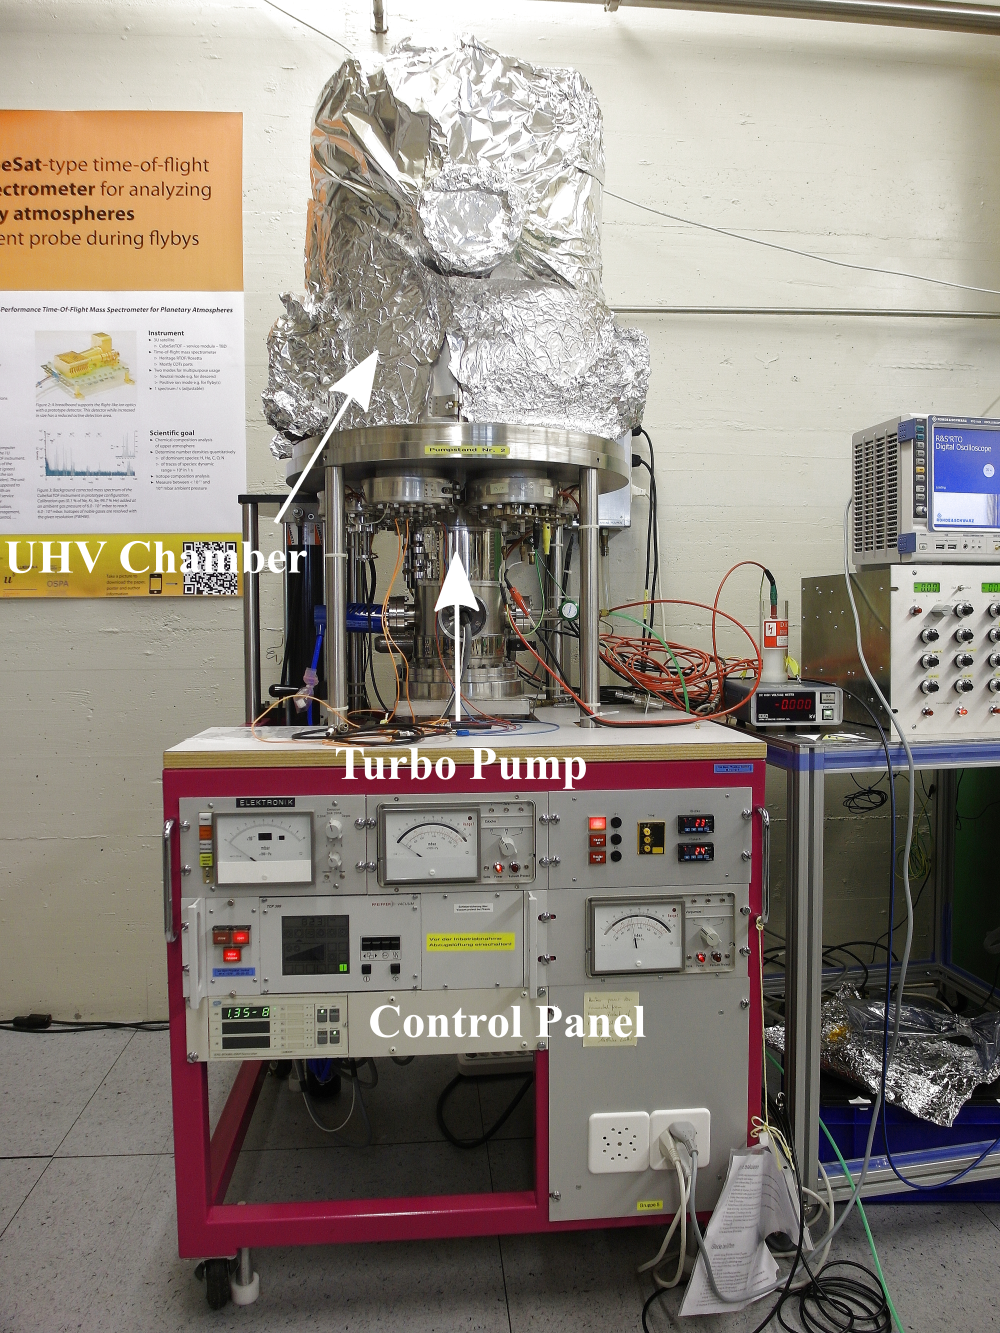
\includegraphics[width=0.8\textwidth]{Bilder/Galerie_Setup/Pumpstand2_midres.png}
	\end{subfigure}
	\begin{subfigure}{.5\textwidth}
	\centering
	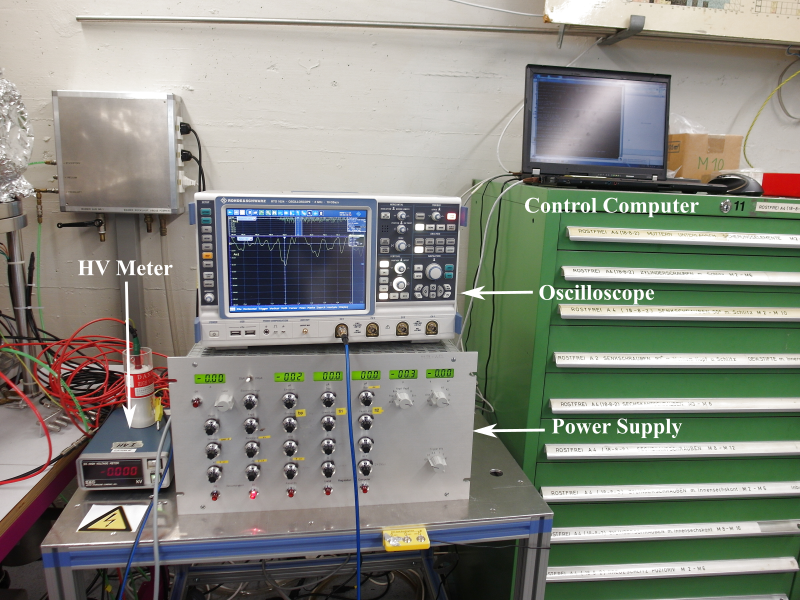
\includegraphics[width=\textwidth]{Bilder/Galerie_Setup/Pumpstand_PSOszi.png}
	\end{subfigure}
	\caption{Left: Pumpstand nr. 2. Right: Power supply, oscilloscope and control computer for the stand-alone tests of the detector. The signal on the oscilloscope is a noise signal.}
	\label{fig:Pumpstand2}
	\end{figure}
	\end{comment}


